\documentclass[a5paper]{article}
\usepackage[a5paper, top=17mm, bottom=17mm, left=17mm, right=17mm]{geometry}
\usepackage[utf8]{inputenc}
\usepackage[T2A,T1]{fontenc}
\usepackage[colorlinks,filecolor=blue,citecolor=green,unicode,pdftex]{hyperref}
\usepackage{cmap}
\usepackage[english,russian]{babel}
\usepackage{amsmath}
\usepackage{amssymb,amsfonts,textcomp}
\usepackage{color}
\usepackage{array}
\usepackage{hhline}
\hypersetup{colorlinks=true, linkcolor=blue, citecolor=blue, filecolor=blue, urlcolor=blue, pdftitle=1, pdfauthor=, pdfsubject=, pdfkeywords=}
% \usepackage[pdftex]{graphicx}
\usepackage{graphicx}
% \usepackage{epigraph}
% Раскомментировать тем, у кого этот пакет есть. Шрифт станет заметно красивее.
%\usepackage{literat}
\usepackage{indentfirst}
\usepackage{multirow}

\sloppy
\pagestyle{plain}
%\pagestyle{empty}

\title{Поддержка жестов мышью в мета-CASE-системах}

\author{М.С. Осечкина \and Т.А. Брыксин \and Ю.В. Литвинов}
\date{}
\begin{document}

\maketitle
\thispagestyle{empty}

\begin{quote}
\small\noindent
Статья рассматривает подходы к поддержке жестов мышью в создаваемых с помощью мета-CASE-инструментария предметно-ориентированных языках визуального моделирования. Приводится численное сравнение алгоритмов распознавания, не использующих предварительное обучение. Делаются выводы о применимости данного класса алгоритмов для повышения эффективности и удобства работы проектировщика, пользующегося визуальным редактором, построенным в мета-CASE-системе. Предложенный подход реализован в мета-CASE-системе QReal.
\end{quote}

\section*{Введение}
Одной из особенностей разработки, управляемой моделями (model-driven development, MDD~\cite{mde}), является активное использование визуальных языков. Практически все действия, выполняемые в CASE-средствах или других используемых инструментах так или иначе сводятся к манипуляциям над элементами этих языков и связями между ними. 

Эффективность любого используемого инструмента определяется тем, насколько удобно и быстро он позволяет выполнять те операции, для которых предназначен. В процессе разработки моделей одними из наиболее часто выполняемых действий над объектами на диаграммах являются их создание и удаление.  В большинстве CASE-средств для того, чтобы создать нужный объект на диаграмме, необходимо найти его либо на панели инструментов, либо выбрать в меню, а затем указать место на диаграмме, где бы мы хотели этот элемент разместить. Также в большинстве инструментариев возможен вариант создания объектов «перетаскиванием» (drag and drop) их из палитры. При этом надо учитывать, что количество видов диаграмм и объектов в палитре каждой диаграммы может быть довольно большим (например, 13 видов диаграмм в UML 2.2). Не всегда возможно оставить в палитре только специфичные для данного типа диаграмм элементы, поскольку может возникать задача быстрого прототипирования с использованием смешанных диаграмм. То есть даже для такой базовой операции, как создание нового элемента, разработчику нужно совершить не только набор чисто механических действий, но ещё и, скажем, вспомнить, на какой вкладке палитры или в каком меню находится нужный ему элемент, тем самым переключая контекст с продумывания иерархии создаваемых моделей на особенности использования выбранного инструмента. Нам кажется, что данную операцию можно и нужно автоматизировать, причём её нужно сделать максимально удобной для пользователей CASE-средств. 

Оптимизация интерфейса под использование жестов особо актуальна в контексте использования CASE-средства на компьютерах с сенсорными экранами или на электронных досках. Такие устройства активно развиваются и уже вошли в повседневную жизнь, например, Microsoft Surface\footnote{http://www.microsoft.com/surface/}.Примерами использования CASE-средств на таких устройствах может являться применение их в процессе обучения или активного обсуждения на совещаниях~\cite{ideogramic}. 

В данной статье в качестве решения по оптимизации интерфейса рассматривается подход, основанный на жестах мышью. Предлагается с каждым элементом ассоциировать определённый жест мышью, выполненный с каким-либо модификатором (скажем, с зажатой правой кнопкой мыши) и при выполнении этого жеста создавать в данном месте соответствующий объект. Например, если пользователь на диаграмме случаев использования UML рисует круг, у него создаётся случай использования (use case), если рисует актёра --- создаётся элемент ``актёр'' (actor).

Использование визуальных языков общего назначения, таких, как UML, не даёт существенного выигрыша в производительности труда программиста, поэтому всё большую популярность набирают предметно-ориентированные визуальные языки~\cite{theBook, dsm}. Мета-CASE-системы предназначены для быстрого создания языка под конкретную предметную область и порождения CASE-инструмента для работы с этим языком. Одним из примеров мета-CASE-систем является среда QReal~\cite{qreal}, разрабатываемая на кафедре системного программирования СПбГУ. В QReal для быстрой разработки новых редакторов диаграмм имеется метаредактор с графическим редактором формы элементов. Он позволяет создавать метамодели новых языков, описывая имеющиеся на диаграммах элементы и связи между ними, задавать визуальное представление элементов на диаграммах. Созданную метамодель можно скомпилировать в подключаемый модуль и подключить его к QReal прямо в процессе работы.

В последнее время разработкам нетрадиционных подходов к организации человеко-машинного взаимодействия уделяется довольно много внимания, и идея подавать команды программам с помощью жестов мыши уже нашла свое применение во многих приложениях, например, браузер Opera\footnote{http://www.opera.com/}, игры. Некоторые утилиты (такие, как StrokeIt, gMote и др.) даже позволяют внедрить поддержку  жестов мышью в произвольные приложения. Более того, существуют и CASE-системы, использующие подобный подход, например, Visual Paradigm\footnote{http://www.visual-paradigm.com/product/vpuml/}. Но поддержка жестов мышью в таких программах ограничена тем, что набор жестов фиксирован, что недопустимо для расширяемых систем, к которым относятся мета-CASE-системы. В данной статье описывается опыт внедрения жестов мышью в приложение, в котором набор жестов неизвестен априори и может быть расширен.

В статье проводится анализ существующих алгоритмов распознавания жестов мышью применительно к использованию в CASE-системах и предлагается алгоритм, позволяющий поддержать жесты мышью для элементов диаграмм в мета-CASE-системе, где набор графических элементов может расширяться динамически. На основе данного алгоритма в среде QReal была создана инфраструктура поддержки жестов.  В статье описываются результаты апробации созданного подхода к поддержке распознавания жестов мышью в среде QReal на примере нескольких графических редакторов из её состава. 

\section{Обзор подходов к распознаванию жестов мышью}

\subsection{Использование жестов мышью в существующих приложениях}

Существует довольно много приложений, в которых использование жестов мыши уже нашло своё применение. Так, например, в веб-браузер Opera встроена поддержка простейших жестов, вызывающих наиболее часто применяемые команды. К примеру, чтобы вернуться к предыдущей странице, можно нажать кнопку ``Back`` в панели браузера, а можно выполнить движение мышью влево при зажатой правой кнопке. Чтобы перейти к следующей странице (кнопка ``Forward``), нужно двигать мышь вправо, для обновления страницы (кнопка ``Reload'') -- вверх-вниз, чтобы открыть новую вкладку -- вниз. Ясно, что при таких абстрактных жестах от алгоритма распознавания не требуется большая точность -- достаточно просто разбить жест на направления и выделить 1-3 вектора наибольшей длины.

В некоторых компьютерных играх жесты позволяют указывать персонажам куда двигаться или заставляют их выполнять какие-то определённые действия. Набор жестов в известных нам приложениях такого рода статичен и не может быть изменён без модификации кода игры.

Также существуют специальные утилиты, с помощью которых можно ввести поддержку жестов мышью в любую программу, такие как strokeIt\footnote{http://www.tcbmi.com/strokeit/}, gMote\footnote{http://www.handform.net/gmote.php}, xstroke\footnote{http://freshmeat.net/projects/xstroke/}, flyGesture\footnote{http://flyingmeat.com/flygesture/}. Их недостаток с точки зрения рассматриваемой задачи состоит в том, что добавляется лишь ограниченное число заранее определённых команд, таких, как сохранение, распечатка, копирование, вставка и т.п. В CASE-системах для полноценной поддержки создания элементов требуется на порядок больше различных жестов. И если в вышеперечисленных утилитах можно обойтись перебором всевозможных путей мыши, по которым вызывается та или иная команда, то в CASE-средстве перебирать придётся слишком много вариантов. Ограничиться простейшими жестами (вверх, вниз, вправо, влево) невозможно, так как объектов слишком много и может возникнуть конфликт между двумя командами, у которых будет один и тот же жест. Возможным решением в таких случаях было бы по жесту предоставлять список команд, из которых пользователь может выбрать. Но если список будет слишком большим или будет вызываться при каждом жесте мышью, то смысл введения жестов пропадает, так как большинство инструментов уже предоставляет пользователю список объектов, которые с помощью операции drag-and-drop можно перетаскивать на рабочее поле.

Отдельно хотелось бы выделить CASE-систему Visual Paradigm, в которой частично реализован предлагаемый в данной статье подход. В Visual Paradigm жесты мышью подразделяются на три типа – жесты, порождающие объект, жесты, вызывающие команду и жесты, создающие связь между объектами. Жесты, порождающие объект и жесты, вызывающие команды задаются набором направлений (вверх, вниз, вправо, влево). Каждая диаграмма имеет отдельный ассоциированный с ней набор жестов, причём жесты имеют не все элементы палитры данной диаграммы, а только наиболее употребимые. Имеется контекстная справка, анимированно показывающая, как рисовать жест. Жесты иногда довольно сильно отличаются от создаваемых ими фигур. Жестов мышью в Visual Paradigm гораздо больше, чем в  утилитах, описанных ранее, но, как и в первых трёх случаях, они жёстко ``зашиты'' в код. 

Аналогичный подход был реализован в инструменте Ideogramic~UML~\cite{ideogramic}, авторы которого особое внимание уделяли распознаванию жестов. Инструмент изначально разрабатывался как среда визуального моделирования для сенсорных экранов и интеллектуальных досок, но возможна работа и с жестами мыши. Версия инструмента, доступная на данный момент, датируется 2002 годом. В рамках же данной работы хотелось бы развить данную идею и предложить расширяемую технологию поддержки жестов мышью в CASE-средствах. 

Отметим, что во всех рассмотренных приложениях реализация распознавания жестов мышью является закрытой, поэтому не анализируется детально в этой работе.

\subsection{Обзор алгоритмов распознавания жестов мышью}
Задача компьютерного распознавания образов не нова --- различные варианты задач идентификации и классификации объектов решаются уже более сорока лет. За это время было разработано множество алгоритмов и подходов к решению самых разных задач распознавания, однако независимо от их класса и предметной области все подходы работают по следующей схеме: 
\begin{itemize}
  \item анализ и/или измерение объектов;
  \item выделение их характеристических признаков;
  \item классификация объектов в соответствии с полученными признаками.
\end{itemize}

\subsubsection{Этап измерения}
Основной задачей первого этапа является выделение траектории жеста. В таких задачах, как, например, распознавание движений по видеосигналу, этот этап может представлять наибольшую сложность, однако, применительно к решаемой задаче построение траектории сводится к отслеживанию перемещения координат курсора мыши, что не представляет сложностей в реализации. Как в случае использования мыши, так и в случае сенсорных экранов и интеллектуальных досок имеется не только путь указателя, но и события, обозначающие начало и конец траектории.

\subsubsection{Выделение признаков}
Большинство существующих алгоритмов распознавания работают с векторами характеристик объектов, которые позволяют абстрагироваться от несущественных для решаемой задачи признаков, например, таких, как пространственное положение и размеры распознаваемого объекта. В нашем случае каждому жесту соответствует траектория движения курсора мыши --- список точек. Однако, использовать списки точек в качестве характеристических векторов не удаётся, так как при переносе или масштабировании жеста их координаты могут меняться довольно сильно. Мы будем рассматривать методы, предлагающие следующее решение проблемы: некоторым образом сопоставим каждому жесту строку символов (которую далее будем называть строкой-ключом) и будем сравнивать не списки точек траекторий, а соответствующие им ключи. Отметим, что закодировать жест строкой символов можно совершенно разными способами, например, рассмотреть как строку бинарное представление набора точек в пути. Наибольший интерес представляют методы построения ключа, которые сохраняют только существенную информацию о жесте, некоторые такие методы и будут рассмотрены далее.

Наиболее очевидным подходом к построению ключа является отслеживание изменений ориентации сегментов ломаной, соответствующей жесту, относительно выбранной системы координат~\cite{chaosAlgorithm}. Участку жеста соответствует угол на плоскости, который попадает в один из диапазонов, а каждому из диапазонов углов ставится в соответствие символ в алфавите (см. рис.~\ref{chaos}). 

\begin{figure} [ht]
  \begin{center}
    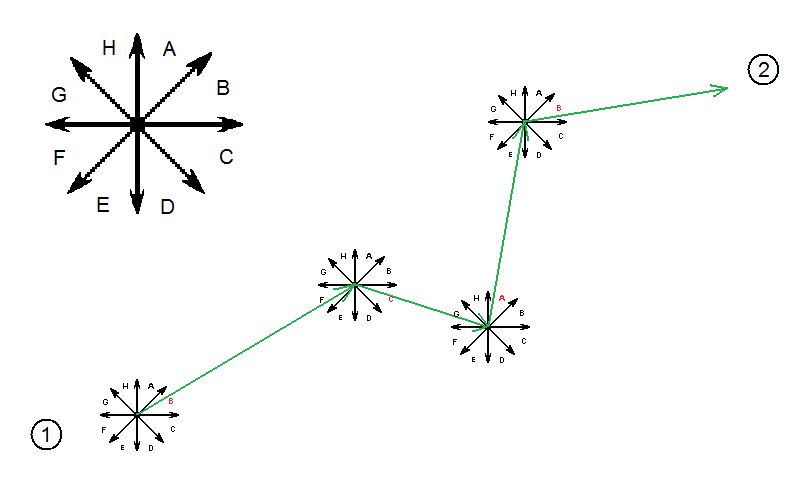
\includegraphics[width=0.9\textwidth, bb=0 0 804 498]{02-chaos.png}
    \caption{Построение ключа по принадлежности направлению}
    \label{chaos}
  \end{center}
\end{figure}

Путь мыши при этом представляется как последовательность символов, соответствующих каждому из направлений. Недостаток этого алгоритма состоит в том, что даже небольшое дрожание руки, породившее короткий отрезок в неправильном направлении, добавит в ключ-строку новые символы, что может привести к ложному распознаванию жеста.

Другой алгоритм предлагает рассматривать не принадлежность направлению, а принадлежность прямоугольнику. Вокруг траектории законченного жеста описывается прямоугольник, каждая сторона которого делится на 8 частей (см. рис.~\ref{squares}). Каждому внутреннему прямоугольнику ставится в соответствие символ алфавита. Строка-ключ жеста будет состоять из символов, соответствующих прямоугольникам, по которым проходит траектория жеста. После удаления подряд идущих одинаковых символов из строки получаем окончательный ключ текущего жеста. 

\begin{figure} [ht]
  \begin{center}
    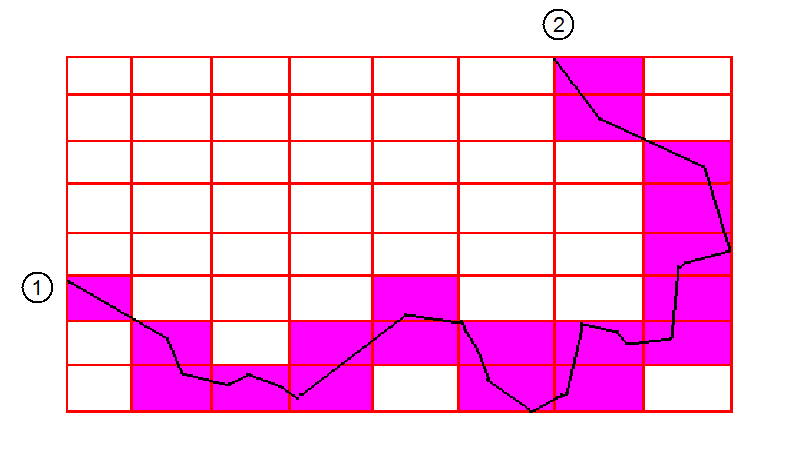
\includegraphics[width=0.8\textwidth, bb=0 0 544 390]{03-squares.png}
    \caption{Построение ключа по принадлежности прямоугольнику}
    \label{squares}
  \end{center}
\end{figure}

Эти алгоритмы хороши тем, что при их использовании не надо масштабировать жест. Подобным фигурам будут соответствовать одни и те же ключи.

Подряд идущие повторяющиеся символы можно не удалять, но тогда жест придётся приводить к заранее определённому стандартному размеру. Но в этом случае при уменьшении некоторых ломаных может оказаться, что некоторые их части становятся слишком маленькими и могут быть на этапе фильтрации приняты за шум.

\subsubsection{Классификация объектов}
Для различения объектов часто используются специальные математические модели, называемые классификаторами. Получая на вход вектор признаков, классификатор сообщает, к какому классу объектов принадлежит данный объект. При этом классификатор не использует информации о способе построения вектора признаков, так что использование классификаторов в целом не зависит от вида решаемой задачи, и существующие классификаторы могут быть использованы для распознавания жестов мышью. 

Среди используемых подходов к классификации наибольшей популярностью в задачах распознавания пользуются такие математические модели, как искусственные нейронные сети~\cite{neuronet1, neuronet2, neuronet3}, скрытые марковские модели~\cite{hmm1, hmm2, hmm3}, а также классификаторы, получаемые обучением с помощью, например, метода опорных векторов~\cite{svm1, svm2} или алгоритмов AdaBoost/FloatBoost~\cite{boosting1, boosting2}. Принцип работы у всех этих классификаторов примерно одинаковый --- вначале осуществляется фаза обучения, на которой классификатору на вход подаётся набор эталонных объектов, соответствующих каждому классу. В рабочем режиме обученный классификатор сопоставляет входные вектора признаков классу, соответствующему данным объектам.

Наличие этапа обучения для нашей задачи недопустимо, поскольку в процессе метамоделирования новые сущности могут появляться довольно часто, а обучение требует наличия большой базы примеров (например, набора типичных траекторий для каждого жеста). Такую базу невозможно создать в короткие сроки при быстрой разработке предметно-ориентированного языка. Данное ограничение является довольно серьёзным и, к сожалению, не позволяет нам использовать данный вид классификаторов для решения поставленной задачи. Существует несколько открытых реализаций обучаемых классификаторов, например, библиотека AME Patterns\footnote{http://ame4.hc.asu.edu/amelia/patterns/}, но, по указанным причинам, в данной статье мы не будем их рассматривать.

Другим часто используемым в распознавании образов подходом к классификации объектов является так называемая задача поиска ближайшего соседа~\cite{nns1, nns2}, заключающийся в отыскании среди множества элементов, расположенных в некоем метрическом пространстве (в общем случае, многомерном), элементов, близких к заданному, согласно некоторой функции близости, задаваемой статически (в отличие от алгоритмов, основанных на обучении, где функция близости меняется в процессе обучения). В случае представления траекторий строками из некоторого алфавита можно использовать много различных функций близости, но на точность распознавания они влияния не оказывают, поскольку не должны учитывать физические свойства векторов признаков. Наиболее известной такой функцией является расстояние Левенштейна, которое определяется как минимальное количество операций вставки одного символа, удаления одного символа и замены одного символа на другой для превращения одной строки в другую~\cite{levenshtein}. Однако, расстояние Левенштейна обладает следующим недостатком: расстояния между совершенно разными короткими строками оказываются небольшими, а расстояния между похожими длинными словами оказываются значительными. Поэтому обычно используется не само расстояние, а соотношение 

\begin{equation}
\label{levenshtein}
d_{normalized}(s1,s2) = \frac{d(s1,s2)}{min(s1,s2)},
\end{equation}

где d(s1,s2) -- расстояние Левенштейна между строками s1 и s2, а min(s1,s2) -- минимум длин этих строк. Рассматриваемые нами методы построения строки-ключа обладают тем свойством, что незначительно отличающимся жестам обычно соответствуют незначительно отличающиеся строки с точки зрения нормализованного расстояния Левенштейна, поэтому такая функция вполне подходит для наших целей.

\subsubsection{Алгоритм распознавания жестов без генерации строки-ключа}
\label{qtAlgorithm}
При создании QReal использовался инструментарий Qt\footnote{http://qt.nokia.com/}, разработчиками которого предложен свой алгоритм распознавания жестов мышью, не требующий в процессе работы построения строки-ключа и основанный на анализе изменения направлений участков жеста~\cite{qtGestures}. Рассмотрим шаги алгоритма.
\begin{enumerate}
  \item Фильтрация пути мыши. Работает на этапе формирования пути по данным с мыши и не допускает записи в путь слишком коротких отрезков. Этот шаг необходим, поскольку последующие шаги алгоритма могут работать некорректно, если отрезок в пути слишком короткий, кроме того, это снижает зависимость алгоритма от особенностей аппаратной части.
  \item Сопоставление объекта из списка. Предполагается, что объект в этом алгоритме --- это ломаная.
  \begin{enumerate}
    \item Приближение направлениями. На этом этапе каждый сегмент ломаной приближается одним из заранее определённых базовых направлений. Как правило, их четыре --- вверх, вниз, вправо, влево. Для большей точности количество базовых направлений можно увеличить, при этом удобно брать число, кратное четырём, чтобы четыре базовых направления оставались неизменными, и каждое было биссектрисой двух соседних. При увеличении числа направлений к эталонным жестам можно добавлять сложные многоугольники, стороны которых не обязательно параллельны осям координат, которые было бы невозможно распознать в случае использования только четырёх направлений.
    \item Упрощение списка направлений, заключающееся в том, чтобы найти подряд идущие сонаправленные вектора и объединить их в один вектор, просуммировав длину.
    \item Сопоставление и удаление. Эта часть алгоритма является, пожалуй, наиболее сложной, так как, несмотря на фильтрацию, останутся мелкие сбои вдоль длинных отрезков. На этом шаге полученному списку направлений сопоставляется эталонный жест команды. Если соответствующий эталонный жест не найден, мы удаляем кратчайший отрезок и повторяем попытку. Алгоритм заканчивается, если удалось получить команду, или большая часть первоначального списка направлений была удалена.
  \end{enumerate}
\end{enumerate}

Недостаток этого алгоритма состоит в том, что изменение оставшихся отрезков после удаления самого короткого довольно нетривиально. Чтобы путь не потерял связность, удалить отрезок, не изменив концы соседних с ним, невозможно. Чтобы отрезки сохранили своё направление, придётся менять не только соседние. Например, на рис.~\ref{qt} слева показана часть пути мыши. После удаления самого короткого отрезка с номером 2, переносим отрезок номер 3, тем самым меняя координаты начала отрезка номер 4. Путь преобразуется в траекторию, приведённую на рис.~\ref{qt} справа. Стоит заметить, что при увеличении числа направлений перестраивать путь будет все сложнее. 

\begin{figure} [ht]
  \begin{center}
    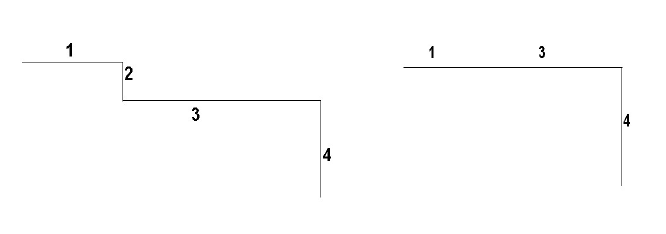
\includegraphics[width=0.8\textwidth, bb=0 0 500 200]{04-qt.png}
    \caption{Объединение участков пути}
    \label{qt}
  \end{center}
\end{figure}

\section{Предлагаемый подход}
\label{rectAlgorithm}
Исходя из рассмотренных алгоритмов распознавания, а также в соответствии со спецификой задачи, был выбран подход, основанный на формировании строки-ключа алгоритмом определения принадлежности прямоугольнику и использовании в качестве классификатора модифицированной функции Левенштейна~(\ref{levenshtein}). Однако, для классификации жестов требуется набор эталонов --- объектов, с которыми сравнивается входной набор признаков при поиске ближайшего соседа. В нашем случае эталонные вектора признаков будут строиться по так называемым ``идеальным жестам'' --- жестам, генерируемым на основе графического представления элементов. 

Для каждого объекта в QReal есть графическое представление, которое задаётся с помощью текстового языка на основе XML (подробнее см. в~\cite{qreal}). Описание элемента представляет собой набор отрезков, каждый из которых определяется координатами начала и конца, и набор окружностей, которые определяются координатами центра и диаметром. В случае с отрезками идеальный путь может быть построен непосредственно, окружности же требуют некоторой предварительной обработки. Дело в том, что система получает сигналы о движении мыши через некоторые короткие промежутки времени, поэтому изображённый пользователем путь представляется не как окружность, а как ломаная с короткими рёбрами. При равномерном движении мыши окружность можно представить как правильный многоугольник. Для достаточно точного распознавания можно выбрать для приближения окружности многоугольник с шестнадцатью вершинами (шестнадцатиугольник выбирается так, что точки с минимальной и максимальной абсциссой и ординатой являются его вершинами). Такое приближение позволяет с достаточной точностью распознавать окружности, как будет показано далее.

Таким образом, для каждого объекта можно выделить набор вершин (концы всех отрезков и точки на окружности) и рёбер (отрезки) и построить по ним граф, соответствующий объекту. Такой граф, поскольку он повторяет линии изображения фигуры, будет визуально похож на фигуру, ему соответствующую. Начальную точку жеста и порядок рисования пользователю придётся запомнить, и при построении ``идеального жеста'' порядок рисования может быть выбран произвольно (в нашей реализации он зависит от порядка элементов в описании фигуры). Построение ``идеального жеста'' основано на понятии эйлерова пути графа --- пути, проходящего по всем рёбрам графа, причём по каждому из них только по одному разу. Эйлеров путь зависит от того, в каком порядке описаны графические элементы (окружности и отрезки) объекта в метамодели. По этому списку генерируется список рёбер графа и осуществляется обход графа в глубину. Если в полученном графе объекта эйлеров путь не существует, добавим несколько рёбер так, чтобы эйлеров путь существовал. Добавлять будем кратчайшее из возможных рёбер, связывающих два эйлеровых подграфа, пока не получим эйлеров путь. Если кратчайших рёбер несколько, может быть добавлено любое, например, для элемента с графическим изображением в виде креста добавленное ребро может быть любым из четырёх рёбер, достраивающих граф до полного. В рассматриваемой реализации добавление определяется порядком, в котором перечислены рёбра в описании графического изображения. Полученный эйлеров путь и будем считать ``идеальным жестом'' для данного объекта. 

Так как данный алгоритм генерации ``идеального жеста'' имитирует реальный путь мыши, полученный в процессе список ``идеальных жестов'' подходит для любого алгоритма распознавания. Что очень удобно, так как не приходится для каждого нового алгоритма задавать вручную список эталонов --- достаточно просто предоставить список ``идеальных жестов'' алгоритму распознавания для последующего сравнения.

Общая схема процесса распознавания мышиного жеста такова.

\begin{itemize}
  \item CASE-система получает сигналы о том, что пользователь зажал правую кнопку мыши и перемещает курсор, и сохраняет координаты положения курсора через равные промежутки времени. Жест считается завершённым, когда пользователь отпускает кнопку мыши.
  \item Осуществляется сглаживание полученной траектории. Этот шаг необходим, так как различное оборудование дает разную точность при получении позиции курсора. Кроме того, если учитывать все дрожания руки, придётся усложнять следующий шаг --- сопоставление объекта: каждому объекту будет соответствовать слишком много разных вариантов пути мыши.
  \item Списку точек сопоставляется строка в соответствии с алгоритмом, отражённым на рис.~\ref{squares}.
  \item С помощью модифицированного алгоритма Левенштейна находится идеальный ключ, расстояние $d_{normalized}$~(\ref{levenshtein}) между которым и сгенерированным по нарисованному жесту наименьшее. Если ключ достаточно близок к идеальному, на диаграмме создаётся объект, соответствующий этому ключу.
\end{itemize}

\subsection{Описание функциональности}
В предложенной реализации список ``идеальных жестов'' создаётся на основе графических представлений элементов на этапе генерации соответствующего визуального редактора.

Далее, чтобы создать определённый элемент, пользователь CASE-системы зажимает правую кнопку мыши и делает соответствующий жест. Для того, чтобы пользователь мог контролировать процесс рисования, система показывает получающийся путь (см. рис.~\ref{drawing}, рисуемый жест заведомо укрупнён).

\begin{figure} [ht]
  \begin{center}
    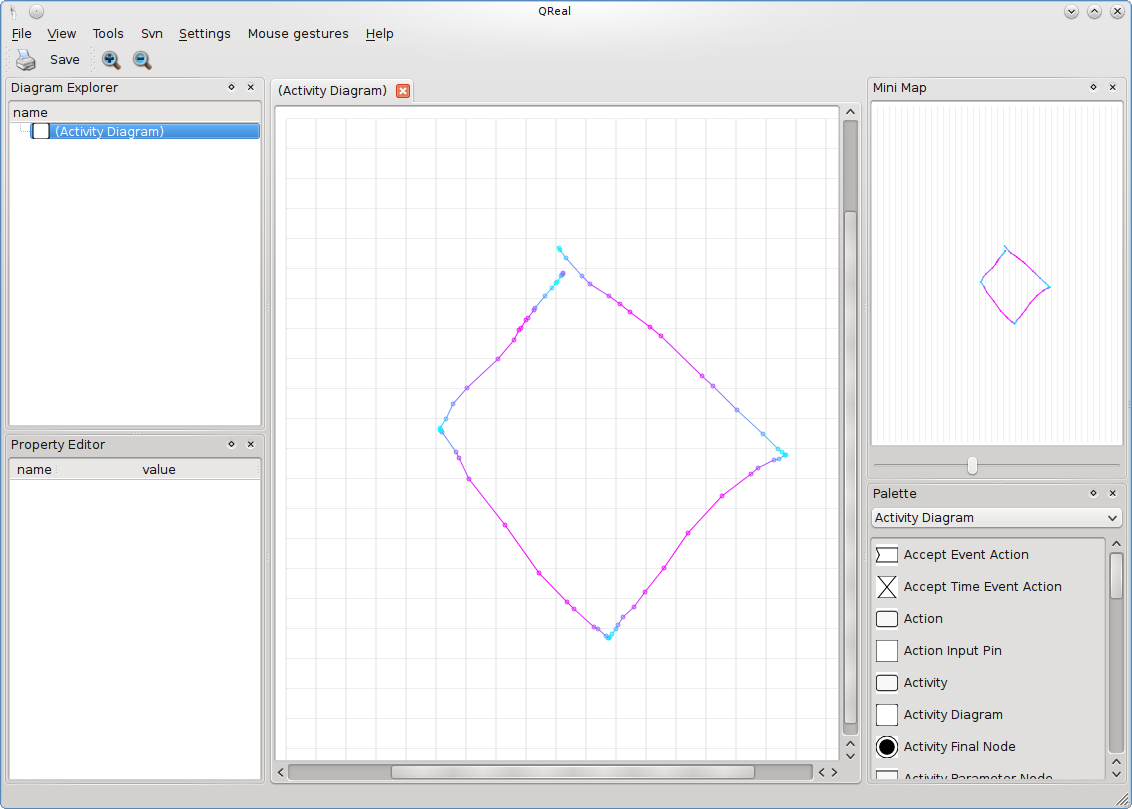
\includegraphics[width=0.8\textwidth, bb=0 0 800 600]{05-drawing.png}
    \caption{Рисование жеста для элемента Decision Node диаграммы активностей UML}
    \label{drawing}
  \end{center}
\end{figure}

После того, как пользователь отпускает правую кнопку мыши, жест считается завершённым и QReal строит ключ-строку в соответствии с алгоритмом, отражённым на рис.~\ref{squares}. По тому, какая диаграмма была активна в момент рисования жеста, определяется нужный графический редактор, у него запрашивается список ``идеальных жестов'' всех описанных в нем элементов и считается расстояние Левенштейна между каждым из них и нарисованным. Тот элемент, расстояние до которого будет минимальным (но в то же время достаточно небольшим, чтобы исключить ложно-позитивные срабатывания для совсем непохожих жестов), создаётся в центре изображённого пользователем жеста, а сама ломаная исчезает. 

Возникает проблема похожести жестов: ``идеальный жест'' генерируется по описанию графического представления объекта, и если графически объекты похожи, то и жесты для них будут похожи. В пределах одного редактора малоразличимые ``идеальные жесты'' даётся возможность редактировать вручную: например, вводится операция вращения, и некоторые жесты предлагается рисовать по часовой стрелке, а некоторые --- против. В данный момент решение о вращении ``идеального жеста'' принимает разработчик визуального языка при описании этого элемента в метамодели. 

Однако, одной только операции вращения иногда оказывается мало, так как внутри одного языка может быть довольно много визуально похожих элементов. В таком случае после рисования жеста CASE-система предлагает выбрать нужный элемент из выпадающего меню, появляющегося после завершения жеста. Элементов в таком меню будет значительно меньше, чем во всей палитре редактора.

Данный подход был также расширен и на создание ассоциаций на диаграммах. Так как у связей между объектами графическое представление как таковое отсутствует (стиль начертания линий, а также стиль заливки и форма стрелок для наших целей подходят плохо), логично предположить, что жестом, порождающим такую ассоциацию, будет кривая, соединяющая два нужных элемента. Если QReal замечает жест, начинающийся и заканчивающийся на уже существующих на диаграмме объектах, то через API доступа к плагинам получается список ассоциаций, допустимых между объектами данных типов, и отображается в выпадающем меню, аналогично рассмотренному выше случаю создания элементов. После выбора одного из пунктов меню между данными объектами создаётся соответствующая связь (отметим, что если в данном списке связей находится всего одна ассоциация, она создаётся сразу же после завершения жеста).

Пользователь может просмотреть список жестов, доступных для данной диаграммы. При выборе соответствующего пункта меню в отдельной вкладке будут показаны все доступные жесты и анимированно изображено, как каждый жест надо рисовать. Анимация рисуется по ``идеальному жесту''.

\subsection{Реализация}

Общая схема создания визуального языка с поддержкой жестов мышью в QReal на данный момент такова.
\begin{itemize}
  \item В метаредакторе описывается абстрактный синтаксис языка, для каждого элемента задаётся его конкретный синтаксис с помощью редактора фигур.
  \item По модели, созданной в метаредакторе, генерируется xml-файл метамодели языка, включающий в себя описания формы фигур.
  \item xml-файл метамодели открывается в отдельном приложении, автоматически строящем по формам фигур ''идеальные жесты'' как последовательность точек ``идеального'' пути мыши и сохраняющем построенные ``идеальные жесты'' в этот же xml-файл как атрибуты элементов.
  \item xml-файл компилируется компилятором метамоделей в плагин редактора языка, при этом генерируются методы, возвращающие ``идеальный жест'' для каждого элемента.
\end{itemize}
Планируется интегрировать генератор ``идеальных жестов'' с метаредактором и редактором фигур, чтобы, во-первых, ``идеальные жесты'' добавлялись в метамодель полностью автоматически при сохранении, а во-вторых, была возможность редактировать ``идеальный жест'' визуально.

Распознавание жестов мышью в ядре системы реализовано следующим образом.
\begin{itemize}
  \item Когда пользователь создаёт новую диаграмму или переключается на уже существующую, для неё создаётся объект-распознаватель, который запрашивает у плагина редактора языка диаграммы список ``идеальных жестов'', к ней относящихся. Для каждого ``идеального жеста'' вызывается алгоритм построения ключа, построенные ключи сохраняются вместе с идентификаторами элементов, к которым они относятся. Заметим, что на данный момент QReal позволяет создавать на диаграмме элементы разных языков, но каждая диаграмма, тем не менее, относится к одному конкретному языку, его жесты и используются распознавателем.
  \item Когда пользователь зажимает правую кнопку мыши, в распознаватель последовательно передаются точки пути мыши, по которым он строит путь и вычисляет центр рисуемой фигуры.
  \item Когда пользователь отпускает правую кнопку, распознаватель вызывает алгоритм построения ключа, передавая ему реальный путь мыши, после чего ищет наиболее похожий на него идеальный ключ. Используемый алгоритм построения ключа от распознавателя не зависит, так что он может быть легко заменён другим алгоритмом.
  \item Если жест считается распознанным, на диаграмме создаётся новый элемент, в позиции, определяемой центром жеста.
\end{itemize}

\subsection{Апробация}

Результативность предлагаемого алгоритма распознавания была измерена на элементах редактора диаграммы активностей UML 2. Для этого был реализован специальный инструмент, который работал по следующему принципу:
\begin{itemize}
  \item Загружается набор ``идеальных жестов'' из .xml-файла. ``Идеальные жесты'' генерировались автоматически при компиляции соответствующего редактора в QReal.
  \item Пользователь выбирает один из ``идеальных жестов'' в списке и начинает рисовать жесты, соответствующие выбранному.
  \item Пути нарисованных жестов сохраняются в .xml-файл. Тестовый инструмент умеет загружать существующие пути из этого файла и дополнять их вновь нарисованными, таким образом, можно обеспечить параллельность формирования базы жестов.
  \item Когда формирование базы жестов завершено, на каждом из сохранённых жестов запускаются тестируемые алгоритмы. Сравнение проводилось между алгоритмом, описанным в~\ref{qtAlgorithm} и предлагаемым нами алгоритмом.
\end{itemize}

Результаты тестирования приведены в~\ref{experimentsTable}. Для каждого элемента было нарисовано около 130 жестов, жесты рисовало 3 человека.

\begin{table} [ht]
\begin{center}
  \label{experimentsTable}
  \fontsize{7}{18}
  \selectfont
  \begin{tabular} {| c | c || c | c | c || c | c | c || c | c | c ||}
    \hline
    \multirow{2}{*}{№} & \multirow{2}{*}{Идеальный жест}                           & \multicolumn{3}{c||}{rect} & \multicolumn{3}{c||}{qt}          & \multicolumn{3}{c||}{dir}  \\
    \cline{3-11}
      &                                                                               & +       & ?      & -       & +          & ?         & -        & +       & ?         & -     \\ \hline     
    1 &  \scalebox{0.5}{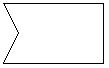
\includegraphics[scale=0.5, bb=0 0 109 68]{gesture1.png}}     & 26\%    & 67\%   & 7\%     & 15\%       & 1\%       & 83\%     & 17\%    & 60\%      & 23\%  \\ \hline
    2 &  \scalebox{0.5}{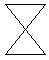
\includegraphics[scale=0.5, bb=0 0 49 60]{gesture2.png}}      & 96\%    & 1\%    & 3\%     & 3\%        & 0\%       & 97\%     & 9\%     & 71\%      & 20\%  \\ \hline
    3 &  \scalebox{0.5}{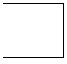
\includegraphics[scale=0.5, bb=0 0 67 64]{gesture3.png}}      & 93\%    & 1\%    & 6\%     & 98\%       & 0\%       & 2\%      & 57\%    & 41\%      & 2\%   \\ \hline
    4 &  \scalebox{0.5}{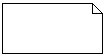
\includegraphics[scale=0.5, bb=0 0 105 56]{gesture4.png}}     & 60\%    & 39\%   & 1\%     & 15\%       & 18\%      & 67\%     & 51\%    & 16\%      & 33\%  \\ \hline
    5 &  \scalebox{0.5}{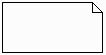
\includegraphics[scale=0.5, bb=0 0 106 55]{gesture5.png}}     & 98\%    & 2\%    & 0\%     & 45\%       & 0\%       & 55\%     & 58\%    & 6\%       & 36\%  \\ \hline
    6 &  \scalebox{0.5}{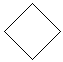
\includegraphics[scale=0.5, bb=0 0 63 62]{gesture6.png}}      & 96\%    & 1\%    & 3\%     & 2\%        & 19\%      & 79\%     & 4\%     & 72\%      & 24\%  \\ \hline
    7 &  \scalebox{0.45}{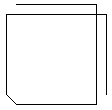
\includegraphics[scale=0.35, bb=0 0 112 110]{gesture7.png}}  & 75\%    & 24\%   & 1\%     & 82\%       & 2\%       & 16\%     & 40\%    & 40\%      & 20\%  \\ \hline
    8 &  \scalebox{0.5}{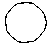
\includegraphics[scale=0.5, bb=0 0 52 47]{gesture8.png}}      & 98\%    & 2\%    & 0\%     & 18\%       & 3\%       & 79\%     & 50\%    & 39\%      & 11\%  \\ \hline
    9 &  \scalebox{0.5}{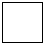
\includegraphics[scale=0.5, bb=0 0 46 46]{gesture9.png}}      & 85\%    & 1\%    & 14\%    & 79\%       & 0\%       & 21\%     & 69\%    & 29\%      & 2\%   \\ \hline
    10&  \scalebox{0.5}{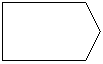
\includegraphics[scale=0.5, bb=0 0 103 64]{gesture10.png}}    & 93\%    & 5\%    & 2\%     & 0\%        & 67\%      & 33\%     & 33\%    & 47\%      & 20\%  \\ \hline
  \end{tabular}
  \caption{Результаты сравнения алгоритмов}
\end{center}
\end{table}

\newpage

Условные обозначения: \\
``rect'' --- алгоритм с выделением признаков методом прямоугольников, предлагаемый в данной статье (см. \ref{rectAlgorithm}).\\
``qt'' --- алгоритм, рассмотренный в \ref{qtAlgorithm}. \\
``dir'' --- алгоритм, основанный на отслеживании изменения направлений (см.~\ref{chaos}). \\
``+'' --- жест распознан. \\
``-'' --- жест не распознан. \\
``?'' --- ложно-позитивное распознавание. \\

Элементы 4 и 5 в таблице имеют одинаковое графическое представление, поэтому для одного из них при генерации ``идеальных жестов'' была применена операция вращения. Жесты для элемента 4 рисовались по часовой стрелке, а для элемента 5 --- против часовой.

Как видно из таблицы, предлагаемый нами алгоритм в большинстве случаев работает лучше, чем два остальных рассмотренных алгоритма. Алгоритм \textit{qt} показывает низкое качество распознавания фигур, содержащих в себе наклонные линии, потому что они приближаются горизонтальными и вертикальными. Фигуры, которые наклонных линий в себе практически не содержат, распознаются этим алгоритмом практически идеально. Алгоритм \textit{dir} корректно распознал несколько больше жестов, чем алгоритм \textit{qt}, однако, высокий процент ложных срабатываний делает его малоприменимым на практике. Связано это с тем, что для этого алгоритма требуется дополнительная фильтрация для учёта похожих направлений: идеальная прямая породит ключ, состоящий из одного символа, а та же прямая с шумом, вызванным, например, дрожанием руки, породит сложный и длинный ключ, сильно отличающийся от идеального. Таким образом, при реализации приходится выбирать между большим количеством ложных срабатываний и приемлемым количеством срабатываний правильных, или большим процентом жестов, не распознанных вовсе.

Алгоритм \textit{rect} таких проблем не имеет, однако, для некоторых элементов так же недопустимо высок процент ложных срабатываний. Например, жест 1 часто путался с жестом 10, алгоритмом \textit{qt} же он практически не распознаётся. 

Заметим, что приближение окружности правильным шестнадцатиугольником обеспечивает достаточную точность распознавания (98\% для алгоритма \textit{rect}), таким образом, более точного приближения окружности ломаными можно не делать.

\subsection{Выводы}
Пробная эксплуатация этого алгоритма в системе показала, что данный подход в предложенном варианте ограниченно применим на практике. Так, создание ассоциаций с помощью жестов действительно показало себя удобным и реально повышающим производительность труда проектировщика. Однако, для достаточно большого набора фигур в палитре точность распознавания реализованного алгоритма (и рассматриваемых аналогов) оказывается недостаточной. Связано это, по нашему мнению, с тем, что для CASE-систем существует некий порог приемлемой точности распознавания жестов. Если алгоритм обеспечивает точность распознавания выше этого порога, то использование жестов мышью оказывается более удобным и эффективным, чем перетаскивание элементов с палитры, если нет, то пользователю придётся потратить больше усилий на рисование фигуры. Данная проблема усугубляется тем, что в CASE-системах требуется распознавать достаточно много (порядка десятков) достаточно похожих жестов, и если для простых приложений, где требуется распознавать единицы жестов, данные алгоритмы могут обеспечить достаточное качество распознавания, в CASE-системах этого добиться не удаётся.

Однако, в случае использования CASE-средств на компьютерах с сенсорными экранами или на электронных досках данный подход кажется нам имеющим право на практическое применение, потому что пером на экране рисовать проще, чем мышью, а перетаскивать элементы сложнее. Кроме того, если набор элементов, для которых будут задаваться жесты, ограничить наиболее часто используемыми и не пытаться распространять подход на все присутствующие в палитре элементы, точность распознавания можно повысить до приемлемой.

\section{Заключение}
Подход, предлагаемый в этой статье, был реализован и внедрён в CASE-систему QReal. На основе проведённых экспериментов были сделаны выводы о применимости описанного в статье решения в расширяемых CASE-системах.
\begin{itemize}
  \item Использование хорошо зарекомендовавших себя в других областях подходов к классификации объектов, основанных на обучении, оказалось затруднительно в системах, где набор распознаваемых объектов может меняться динамически.
  \item Используемый нами классификатор, не использующий обучение, показал недостаточную для практического использования точность распознавания. Однако, при определённых ограничениях рассматриваемые в статье методы обеспечивают приемлемое качество распознавания: во-первых, можно сократить количество классов  распознаваемых объектов, во-вторых, можно использовать более точные, чем мышь, механизмы рисования жеста, например, сенсорные экраны или ``интеллектуальные классные доски''. При подобных ограничениях использование жестов мышью в качестве инструмента для создания новых элементов показало себя достаточно удобным.
\end{itemize}

\pagebreak

\begin{thebibliography}{9001}
  \bibitem{levenshtein} В.И. Левенштейн. Двоичные коды с исправлением выпадений, вставок и замещений символов // Доклады Академий Наук СССР, 1965. 163.4: С. 845-848
  \bibitem{dsm} А.А. Павлинов, Д.В. Кознов, А.Ф. Перегудов и др., О средствах разработки проблемно-ориентированных визуальных языков. // Системное программирование. Вып. 2. СПб.: Изд-во СПбГУ. 2006,  С. 116-141.
  \bibitem{qreal} А.Н. Терехов, Т.А. Брыксин, Ю.В. Литвинов и др., Архитектура среды визуального моделирования QReal. // Системное программирование. Вып. 4. СПб.: Изд-во СПбГУ. 2009, С. 171-196
  \bibitem{svm1} Aizerman, M., Braverman, E., Rozonoer, L., Theoretical Foundations of the Potential Function Method in Pattern Recognition Learning // Automation and Remote Control 25, 1964, P. 821–837.
  \bibitem{neuronet1} Bishop, C., Neural Networks for Pattern Recognition // Oxford: Oxford University Press, 1995, 482 pp.
  \bibitem{chaosAlgorithm} Brun, D., Mouse Gesture Recognition // ByteArray.org Actionscript 3 Experiments. URL: http://www.bytearray.org/?p=91 
  \bibitem{svm2} Catanzaro, B., Sundaram N., Keutzer K., Fast Support Vector Machine Training and Classification on Graphics Processors // Proceedings of the 25th International Conference on Machine Learning (ICML 2008) (2008), P. 104-111.
  \bibitem{ideogramic} Damm, C.H., Hansen, K.M., Thomsen, M., Tyrsted, M. Creative Object-Oriented Modelling: Support for Creativity, Flexibility, and Collaboration in CASE Tools // Proceedings of ECOOP'2000, 2000, P. 27-43
  \bibitem{neuronet3} Faaborg, A., Using Neural Networks to Create an Adaptive Character Recognition System // Cornell University, Ithaca, NY, 2002, 23 pp.
  \bibitem{boosting1} Freund, Y., Schapire, R., A Short Introduction to Boosting // Japanese Society for Artificial Intelligence, Vol. 14, No. 5. (1999), P. 771-780.
  \bibitem{theBook} Kelly, S., Tolvanen, J. Domain-Specific Modeling: Enabling Full Code Generation // Wiley-IEEE Computer Society Press. 2008. 448 pp.
  \bibitem{boosting2} Li, S., Zhang, Z., FloatBoost Learning and Statistical Face Detection // IEEE Transactions on Pattern Analysis and Machine Intelligence, Vol. 26, No. 9. 2004. P. 1112-1123.
  \bibitem{nns1} Potamias, M., Athitsos, V., Nearest Neighbor Search Methods for Handshape Recognition // Proceedings of the 1st international conference on PErvasive Technologies Related to Assistive Environments (PETRA), Vol. 282. 2008, P. 30-38
  \bibitem{hmm1} Rabiner, Lawrence R., A Tutorial on Hidden Markov Models and Selected Applications in Speech Recognition // Proceedings of the IEEE, 1989, P. 257-286.
  \bibitem{neuronet2} Ripley, B., Pattern Recognition and Neural Networks // Cambridge University Press. 1996. 416 pp.
  \bibitem{mde} Schmidt, D. Model-Driven Engineering // IEEE Computer, Vol. 39, No. 2. 2006. p. 25-31. URL: http://www.cs.wustl.edu/\textasciitilde schmidt/PDF/GEI.pdf
  \bibitem{hmm2} Starner, T., Pentland, A., Visual Recognition of American Sign Language Using Hidden Markov Models // International Workshop on Automatic Face and Gesture Recognition. 1995. P. 189-194.
  \bibitem{nns2} Shakhnarovish, Darrell, and Indyk, Nearest-Neighbor Methods in Learning and Vision // MIT Press. 2005. 262 pp.
  \bibitem{qtGestures} Thelin, J., Recognizing Mouse Gestures // Qt Online Reference Documentation, URL: http://doc.trolltech.com/qq/qq18-mousegestures.html 
  \bibitem{hmm3} Vlontzos, J., Kung, S., Hidden Markov Models for Character Recognition // IEEE Transactions on Image Processing, Vol. 1, No. 4. 1992. p. 539-543.
\end{thebibliography}  

\end{document}